\documentclass[10pt, letterpaper]{article}
\usepackage[letterpaper,margin=0.75in]{geometry}
\usepackage{graphicx}
\usepackage{amsmath}
\usepackage{multirow}
\usepackage[table]{xcolor}
\usepackage{listings}
\lstset{basicstyle=\ttfamily}
\usepackage{hyperref}
\hypersetup{
    colorlinks=True,
    linkcolor=blue,
    urlcolor=magenta,
}
\setlength{\parindent}{0pt}
\setlength{\parskip}{5pt}
\renewcommand{\abstractname}{Overview}

\begin{document}

\title{CU Research Computing Allocation Request}
\author{Project Title Here}
\date{}
% Original draft, generated from pre-existing website content, by N. Featherstone, Jan 9, 2018
\maketitle


\begin{abstract}
\noindent Please fill out this template when constructing an allocation request for Summit.  Be sure to address all of the bullet points in this worksheet. If you feel that some of the requested information is not applicable, please note why that is rather than leaving that section out of your request entirely.
\\
\\
\noindent Requests for larger allocations will need more detailed justification. As a general guideline, a request for 300K SU might require a two-page proposal, while a 1M+ SU request might require three to five pages.
\\
\\
\noindent \textbf{If you have questions when preparing this allocation request, please contact rc-help@colorado.edu.  We are happy to provide advice and answer any questions.}

\end{abstract}
\section{Introduction and Summary}\label{sec:intro}
%\begin{center}
%\textit{(Suggested length: X pages)}
%\end{center}
Provide some background information on your proposal in this section.  Particularly:

\begin{itemize}
\item Concise Description - Describe the portion of the Project that this computational work supports.
\item Allocation goals - Describe the anticipated goals for this particular effort as a subset of the Project goals.
\item Duration: indicate if this allocation is for one year or until completion of a nearer-term goal whichever is sooner.
\item Expected follow-up - indicate if this is the final allocation for the Project or if work will likely continue.
\item Supporting grants - indicate funding agencies and grant numbers that support this work (if any).
\end{itemize}



%%%%%%%%%%%%%%%%%%%%%%%%%%%%%%%%%%%%%%%%%%%%%%%%%%%%%%%%%%%%%%%%%%%%%%%%%%%%%%%%%%%%%%%%%%%%%%%
%                                               Computational Details
\section{Computational Details}\label{sec:method}
%\begin{center}
%\textit{(Suggested length: X pages)}
%\end{center}

We use a parallel C++ application for production
and a parallel Python one for analysis.

The products are cross-correlations of continuous seismic records.
The code was compiled using \lstinline{g++} compiler.
As the time of execution is several orders of magnitude
larger that of compilation, the code is compiled with flag

\begin{lstlisting}
-O3 -lfftw3 -lstdc++ -lpthread -fopenmp
\end{lstlisting}

It's not a community model but one developed by our group alone (\url{https://github.com/NoisyLeon/Seed2Cor}).
As for third-party libraries, it uses \lstinline{OpenMP} and \lstinline{FFTW}.
The code does not require the use of a container software.
We run our code on \lstinline{shas} partition, using all the 24 cores on each node. Our application doesn't require large amounts of RAM. Depending on the amount of data we assigned and nodes requested on each run, it typically takes one day to one week for our jobs to run. Our application has well-designed checkpoints, so it can be restarted from a saved state. Our application is very I/O intensive. We typically run our application on \lstinline{shas} partition as our jobs don't require high memory.
We are using CPU alone to do the calculation currently.

The other major application is a parallel inversion code in Python
(\url{https://github.com/NoisyLeon/pyMCinv}).
As it's not memory consuming, the inversion code would be run on \lstinline{shas} partition too. The time cost ranges from several hours up to a week depending on the size of data.

The scaling analysis for these two applications is provided in Figure \ref{fig:scaling}.
The applications are OpenMP parallel applications, so they are run on a single node.
A maximum of 24 cores were used in Figure \ref{fig:scaling},
which is a test run for unit inversion.

\begin{figure}
\centering
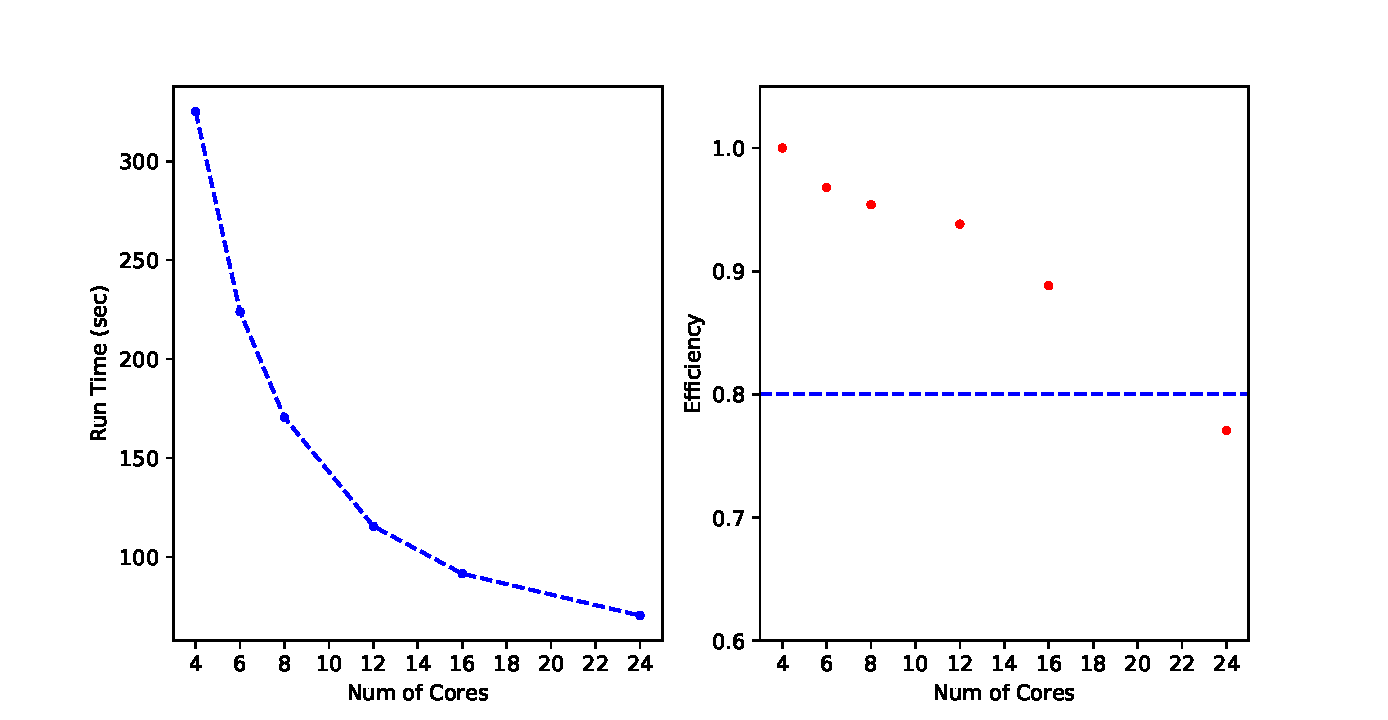
\includegraphics[width=\textwidth, keepaspectratio=true]{scaling.pdf}
\caption{\label{fig:scaling} Sample performance data for a test run. (\textit{a}) Measured run time vs. number of cores.  (\textit{b}) Parallel efficiency vs. numbers of cores.}
\end{figure}

%%%%%%%%%%%%%%%%%%%%%%%%%%%%%%%%%%%%%%%%%%%%%%%%%%%%%%%%%%%%%%%%%%%%%%%%%%%%%%%%%%%%%%%%%%%%%%%
%                                               TIME REQUEST
\subsection{CPU Time Request}\label{sec:request}
%\begin{center}
%\textit{(Suggested length: X pages)}
%\end{center}

Details of our SU request are described in Table \ref{tab:worksheet}.

\begin{table}
\centering
\begin{tabular}{| c | c | c | c | c | c | c|}
\hline
 Job Type           & Node Type & Weight & Jobs  & Cores  & Hours & Total (SU)  \\\hline
Production          & shas      & 1      & 100   & 24     & 160   & 384,000 \\
Inversion           & shas      & 1      & 150   & 24     & 70    & 252,000 \\
Post-processing     & shas      & 1      & 200   & 24     & 2     & 9,600 \\\hline
Grand Total (SU)    & -         & -      &-      & -      &-      & 645,600 \\\hline
\end{tabular}
\caption{\label{tab:worksheet}SU request worksheet.}
\end{table}


%%%%%%%%%%%%%%%%%%%%%%%%%%%%%%%%%%%%%%%%%%%%%%%%%%%%%%%%%%%%%%%%%%%%%%%%%%%%%%%%%%%%%%%%%%%%%%%
%                                               I/O
\section{Data Management}\label{sec:IO}
%\begin{center}
%\textit{(Suggested length: X pages)}
%\end{center}
Our cross-correlation application is very I/O intensive. The typical job that we run each time has around 400 stations with 2 years of continuous data. The continuous data are requested from seismic data management centers, e.g. IRIS (\url{http://ds.iris.edu/ds/}). For raw data of such scale, we expect 700 files, each $\sim$2GB. From the raw data, we extract daily 3-component seismic records and this results in 1,400,000 files, each $\sim$2 MB.
Then cross-correlations are calculated between daily records from different stations, and this will result in around 100,000,000 files, each $\sim$0.2 MB.

The raw data will be removed after the calculation of daily cross-correlations (CC). We will stack the daily CCs to get our stacked CC products. For each job, we expect to output 488,000 stacked files, each $\sim$0.2 MB. All the I/O described here will use \lstinline{/scratch} storage. After we get the stacked CCs, we will make measurements on them and everything else on \lstinline{/scratch} will be removed.

The storage requirements are listed in Table \ref{tab:space}.

The inversion application and other post-processing are not very I/O intensive, and we incorporate Hierarchical Data Format (HDF) to store and organize the results. We use local disk for I/O and for each job we expect 2 or 3 files, each with size of several GB. The stacked CC and inversion results will be migrated to our local computers and we will make backups on our group cluster and local disks.

\begin{table}[h]
\centering
\begin{tabular}{| l | l | l |}
\hline
  Job Type            & Required Space (TB) & Number of Files  \\ \hline
  Requested           & 1.4                 & 700   \\
  Raw                 & 2.8                 & 1,400,000   \\
  Intermediate        & 23                  & 116,800,000 \\
  Result              & 0.1                 & 488,000 \\
\hline
\end{tabular}
\caption{\label{tab:space}Scratch-disk-space requirements by job type.}
\end{table}

%%%%%%%%%%%%%%%%%%%%%%%%%%%%%%%%%%%%%%%%%%%%%%%%%%%%%%%%%%%%%%%%%%%%%%%%%%%%%%%%%%%%%%%%%%%%%%%
%                                               DATA MANAGEMENT
\end{document}
